%% 
%% Author: papian
%% 26/05/18
%% 

\documentclass{bredelebeamer}

\usepackage[cache=false]{minted}
\usemintedstyle{tango}

%%%%%%%%%% C
\newmintinline{c}{
  fontsize=\small,
  breaklines=true
}

\newminted{c}{
  frame=single,
  framesep=2mm,
  fontsize=\scriptsize,
  mathescape
}

\newminted[ccodeline]{c}{
  frame=single,
  framesep=2mm,
  fontsize=\scriptsize,
  mathescape,
  linenos
}


%%%%%%%%% CMAKE
\newminted{cmake}{
  frame=single,
  framesep=2mm,
  fontsize=\scriptsize,
  mathescape,
  linenos,
  breaklines=true
}

% End minted
%%%%%%%%%%%%%%%%%%%%%%%%%%%%%%%%%%%%%%%%%%%%%%%%%%%%%%%%% 

%%%%%%%%%%%%%%%%%%%%%%%%%%%%%%%%%%%%%%%%%%%%%%%% 

\title[OS Project]{Operating System Project}
% Titre du diaporama

\subtitle{An implementation of server-client database using non-blocking operations}
% Sous-titre optionnel

\author{Julmy, S., Papinutto, M. \& Veillard, S.}
% La commande \inst{...} Permet d'afficher l' affiliation de l'intervenant.
% Si il y a plusieurs intervenants: Marcel Dupont\inst{1}, Roger Durand\inst{2}
% Il suffit alors d'ajouter un autre institut sur le modèle ci-dessous.

\institute[UniFr]{University of Fribourg}

\date{30 Septembre 2018}
% Optionnel. La date, généralement celle du jour de la conférence

\subject{Presentation projet OS Group 4 Sylvain Julmy, Michael Papinutto et Sami Veillard}
% C'est utilisé dans les métadonnes du PDF

\logo{
\includegraphics[scale=0.5]{../report/images/unifrlogo.jpg}}

%%%%%%%%%%%%%%%%%%%%%%%%%%%%%%%%%%%%%%%%%%%%%%%%%%%%%%%%%%%%%%%%%%%%% 
\begin{document}

\maketitle

\begin{frame}
  \frametitle{Table of contents}
  \tableofcontents
\end{frame}

\section{Selected Approach}

\begin{frame}
  \frametitle{Multi-threaded Server}
  We selected a multithreaded server as: \\
  \begin{itemize}
  \item Allows to access same data structure
  \item light weight as compared to multi-process server
  \item easier to implement
  \end{itemize}
\end{frame}

\begin{frame}
  \frametitle{To use mutex or not to use mutex}
  Our lock-free implementation allowed us to omit mutex.
  \begin{itemize}
  \item No need to prioritise read or write operations
  \item No deadlock problems
  \item All clients have the same right to access the data structure
  \end{itemize}
\end{frame}

\begin{frame}[fragile]
  \frametitle{Atomic calls}
  Non-blocking operations use atomic operations in order to perform multiple
  operation in one clock cycle. With GCC, we can access them with some
  specific compiler functions
  \footnote{\url{https://gcc.gnu.org/onlinedocs/gcc-4.1.0/gcc/Atomic-Builtins.html}}:
  
  \begin{minted}{c}
    type __sync_fetch_and_add(type *ptr, type value, ...);
    bool __sync_bool_compare_and_swap(
      type* ptr,
      type old_v,
      type new_v,
    ...);
  \end{minted}

  Such operations are in a way an acquire lock - operate - realease lock in
  only one CPU cycle.
\end{frame}

\begin{frame}
  \frametitle{Reversed Split-Ordered Hash-Set}
  
  This implementation offers a rapid access to the data but might require
  slightly more memory than other data structures.
  
  \begin{itemize}
  \item Buckets are linked to a stack as the list grows supplemental bucket
    references are added so that buckets is kept small.
  \item Require to set up a sentinel bucket in order to avoid "corner case" that
    occurs when deleting a reference by a bucket reference.
  \item The sentinel bucket is never deleted.
  \end{itemize}
  
  \begin{figure}
    \centering
    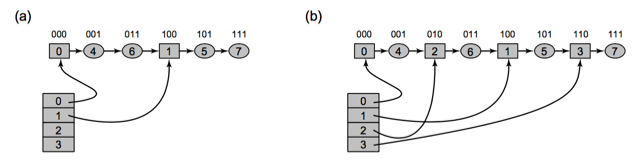
\includegraphics[width=0.9\textwidth]{../report/images/hashsetFig1.png}
    \caption{}
    \label{fig:}
  \end{figure}
\end{frame}

\begin{frame}
  \frametitle{Operation add in this Hash-Set}
  Scheme of the procedure that adds the key 10 to the lock-free hash-set
  \begin{figure}
    \centering
    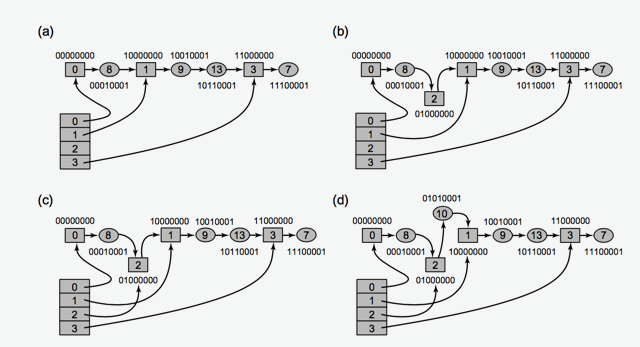
\includegraphics[width=0.9\textwidth]{../report/images/hashsetFig2.png}
  \end{figure}
\end{frame}

\section{Usage and Command Line Interface}

\begin{frame}
  \frametitle{Program Basic Usage}
  
  \begin{tcolorbox}[taborange,tabularx={X|Y}, boxrule=2pt, title=Server usage]
    \verb+TCP Port+ & 5000 (can be changed in file) \\\hline
    \verb+./server+ & server start
  \end{tcolorbox}
  
  \begin{tcolorbox}[tabvert,tabularx={l|Y}, boxrule=2pt, title=Client Start]
    \verb+./ client <server ip address>+ & client start \\\hline
    \verb+./ client -option <server ip address>+ & client start with options
  \end{tcolorbox}
  
\end{frame}

\begin{frame}
  \frametitle{Client Usage and Commands}
  
  \begin{tcolorbox}[taborange,tabularx={X|l}, boxrule=2pt, title=Client Start with options]
    \verb+-?+ \\ \verb+-h+ \\ \verb+--help+ & client command help \\\hline
    \verb+-f <file>+ \\ \verb+--file <file>+ & client start and execute commands in the file \\\hline
    \verb+-F <file1> ... <fileN>+ \\ \verb+--files <file1> ... <fileN>+ & client start and execute commands in the files
  \end{tcolorbox}
  
  \begin{tcolorbox}[tabvert,tabularx={X|Y}, boxrule=2pt, title=Commands in interactive CLI]
    \verb+add <value> or add <key> <value>+ & add a value to the database  \\\hline
    \verb+ls+ & list content (unordered) \\\hline
    \verb+read_v <key>+ & read value from  key \\\hline
    \verb+read_k <value>+ & read key from value \\\hline
    \verb+rm_v <key>+ & delete value from key \\\hline
    \verb+rm_k <value>+ & delete value from key \\\hline
    \verb+update_kv <value> <newvalue>+ & update an entry
  \end{tcolorbox}
  
\end{frame}

\begin{frame}
  \frametitle{Demo}
  \begin{tcolorbox}
      \begin{center}
        DEMO
      \end{center}
  \end{tcolorbox}
\end{frame}

\section{Tests}

\begin{frame}
  \frametitle{Tests scenarios}
  We tested the following scenarios:
  \begin{itemize}
  \item Scenario with collisions : operations that can collide (a client delete a value before another access it).
  \item Scenario without collision : operations that are ordered so that no collision can occur.
  \item Scenario with many clients : several clients with a similar scenario as no-collisions.
  \end{itemize}
\end{frame}

\begin{frame}
  \frametitle{Collision scenarios}
  $11$ clients and $28$ commands ($308$ operations in total)
  
  \begin{tcolorbox}[tabrouge,tabularx={l|X|X|X}, boxrule=3pt]
    & Add & Read & Delete\\\hline
    Number of errors & 0 & 22 & 0 \\\hline
    Percentage of errors & 0\% & 7.14\% & 0\%
  \end{tcolorbox}
  
\end{frame}

\begin{frame}
  \frametitle{No-collision scenarios}
  $8$ clients and $2700$ commands ($21600$ operations in total)
  
  \begin{tcolorbox}[taborange,tabularx={l|X|X|X}, boxrule=3pt]
    & Add & Read & Delete\\\hline
    Number of errors & 0 & 0 & 0 \\\hline
    Percentage of errors & 0\% & 0\% & 0\%
  \end{tcolorbox}
  
\end{frame}

\begin{frame}
  \frametitle{Many clients scenarios}
  
  $32$ clients and $300$ commands ($9600$ operations in total)
  \begin{tcolorbox}[taborange,tabularx={l|X|X|X}, boxrule=3pt]
    & Add & Read & Delete\\\hline
    Number of errors & 0 & 0 & 0 \\\hline
    Percentage of errors & 0\% & 0\% & 0\%
  \end{tcolorbox}
  This last test required more time than the previous one despite the fact that it has half fewer operations
\end{frame}

\section{Conclusion}

\begin{frame}
  \centering
  \textcolor{MidnightBlue}{\Huge Thank's for your attention !}
\end{frame}

\end{document}
